\documentclass[11pt]{article}




\usepackage[sfdefault]{FiraSans} %% option 'sfdefault' activates Fira Sans as the default text font
\usepackage[T1]{fontenc}
\renewcommand*\oldstylenums[1]{{\firaoldstyle #1}}

\usepackage{natbib}
\usepackage[french,english]{babel}
\usepackage{numprint}
\usepackage{multirow}
\usepackage{rotating}
\usepackage{fancyhdr}
\usepackage{booktabs}
\usepackage{multicol}
\usepackage{hyperref}\hypersetup{colorlinks=true}

\usepackage{amsmath,amssymb,amsfonts,textcomp}
\usepackage{color}
\usepackage{calc}
 \setlength{\tabcolsep}{8pt}
\usepackage{setspace}
\onehalfspacing
\usepackage{longtable}
\usepackage{graphicx}
\usepackage[margin=1in]{geometry}
\setlength{\parindent}{0pt}
\usepackage[bottom]{footmisc}
\pagestyle{fancy}
\usepackage{titlesec}
\usepackage{lipsum}
\usepackage{cancel}
\usepackage{multicol}

\usepackage{amsmath,amssymb}
\usepackage{lmodern}
\usepackage{iftex}
\ifPDFTeX
  \usepackage[T1]{fontenc}
  \usepackage[utf8]{inputenc}
  \usepackage{textcomp} % provide euro and other symbols
\else % if luatex or xetex
  \usepackage{unicode-math}
  \defaultfontfeatures{Scale=MatchLowercase}
  \defaultfontfeatures[\rmfamily]{Ligatures=TeX,Scale=1}
\fi

\titleformat{\section}
  {\normalfont\Large\scshape\bfseries}{\thesection}{1em}{}
  \titlespacing{\section}{0pt}{10pt}{0pt}
\titleformat{\subsection}
  {\normalfont\bfseries}{\thesection}{1em}{}
  \titlespacing{\subsection}{0pt}{6pt}{0pt}
\providecommand{\tightlist}{%
  \setlength{\itemsep}{0pt}\setlength{\parskip}{0pt}}\newenvironment{itemize*}%

  
\lhead{EC200 - Econometrics and Applications}
\rhead{Version: \today}
\setlength\parskip{0.10in}
\begin{document}
\thispagestyle{plain}
\singlespacing


Version: \today \hfill Fall 2021\\
EC200: Econometrics and Applications
%\vspace{1.5cm}
\begin{center}
\Large{\textbf{Lab 1: Introduction to Stata}}\\
\end{center}
\bigskip


%{
%\setcounter{tocdepth}{3}
%\tableofcontents
%}
\hypertarget{materials}{%
\subsection*{Materials}\label{materials}}
\addcontentsline{toc}{subsection}{Materials}

\begin{itemize}
\tightlist
\item
  \href{../materials/driving_2004.dta}{\texttt{driving\_2004.dta}}
\end{itemize}

\hypertarget{objectives}{%
\subsection*{\texorpdfstring{Objectives\footnote{This lab draws heavily
  on Anne Fitzpatrick's (UMass-Boston) excellent materials.}}{Objectives}}\label{objectives}}
\addcontentsline{toc}{subsection}{Objectives}

By the end of this tutorial you should be able to complete the following
tasks in Stata:

\begin{itemize}
\item
  Identify key areas of the Stata interface
\item
  Open a data file
\item
  Summarize and tabulate data
\item
  Create and save a log file
\item
  Open, view, and save a data file
\item
  How to get help with Stata
\end{itemize}

If you need more help, check out \href{/bonus/stata-resources}{Stata
Resources}.

\hypertarget{general-command-structure}{%
\subsection*{General command structure}\label{general-command-structure}}

\texttt{do\ \{something\}\ ...\ with\ \{variable(s)\ x\}...if\ \{something\ is\ true..\},\ options}

\hypertarget{key-commands}{%
\subsubsection*{Key commands}\label{key-commands}}
\addcontentsline{toc}{subsubsection}{Key commands}

\begin{longtable}[]{@{}lr@{}}
\toprule
command & description \\
\midrule
\endhead
\texttt{log\ using\ logfile1.log} & open and log using
\texttt{logfile1.log} \\
\texttt{log\ close} & close log \\
\texttt{use\ dataset.dta,\ clear} & open dataset \texttt{dataset.dta},
clear out old one \\
\texttt{describe\ var1\ var2\ ...} & charcteristics of \texttt{var1},
\texttt{var2}, etc. \\
\texttt{browse\ var1\ var2\ ...} & open data browser, display
\texttt{var1,\ var2\ ..} \\
\texttt{lookfor\ text1} & search for \emph{text1} in variable
names/descriptions \\
\texttt{tabulate\ var1} & make a frequency table of \texttt{var1}. \\
\texttt{tabulate\ var1\ var2} & make a cross-tabulation of \texttt{var1}
and \texttt{var2}. \\
\texttt{summarize\ var1} & descriptive statistics for \texttt{var1}. \\
\texttt{summarize\ var1\ ,\ detail} & detailed descriptive statistics
for \texttt{var1}. \\
\texttt{help\ command} & open help files for \texttt{command}. \\
\bottomrule
\end{longtable}

\hypertarget{logic-statements}{%
\subsubsection*{Logic statements}\label{logic-statements}}
\addcontentsline{toc}{subsubsection}{Logic statements}

\begin{longtable}[]{@{}lc@{}}
\toprule
operation & command \\
\midrule
\endhead
and & \& \\
or & \(|\) (vertical bar, on same key as ``/'') \\
& \\
equal to & == \\
not equal to & != \\
& \\
greater than & \textgreater{} \\
less than & \textgreater{} \\
greater than or equal to & \textgreater= \\
less than or equal to & \textless= \\
\bottomrule
\end{longtable}

\begin{itemize}
\tightlist
\item
  \texttt{tab\ bac10\ if\ gdl==1\ \&\ sl70plus\ ==\ 0}

  \begin{itemize}
  \tightlist
  \item
    Tabulates the variable \texttt{bac10} but only if \texttt{gdl}
    equals one \emph{and} \texttt{sl70plus} equals 0
  \end{itemize}
\item
  \texttt{tab\ bac10\ if\ year\ \textgreater{}=2000}

  \begin{itemize}
  \tightlist
  \item
    Tabulates the variable \texttt{bac10} for the years 2000, 2001,
    2002, etc.
  \end{itemize}
\item
  \texttt{tab\ bac10\ if\ year\ !=2000}:

  \begin{itemize}
  \tightlist
  \item
    Tabulates the variable \texttt{bac10} for every year \emph{but} 2000
  \end{itemize}
\item
  \texttt{tab\ bac10\ if\ year\ \textless{}\ 2008\ \&\ year\ \textgreater{}\ 2005}

  \begin{itemize}
  \tightlist
  \item
    Tabulates the variable \texttt{bac10} 2006 and 2007
  \end{itemize}
\item
  \texttt{tab\ bac10\ if\ year\ \textless{}\ 2008\ \textbar{}\ year\ \textgreater{}\ 2005}

  \begin{itemize}
  \tightlist
  \item
    Tabulates the variable \texttt{bac10} is less than 2008 OR greater
    than 2005 (all years!)
  \end{itemize}
\end{itemize}

\hypertarget{hey-stata.-its-nice-to-meet-you}{%
\subsection*{Hey, Stata. It's nice to meet
you}\label{hey-stata.-its-nice-to-meet-you}}

Start by opening Stata. You should have a window that looks something
like this (on a PC):

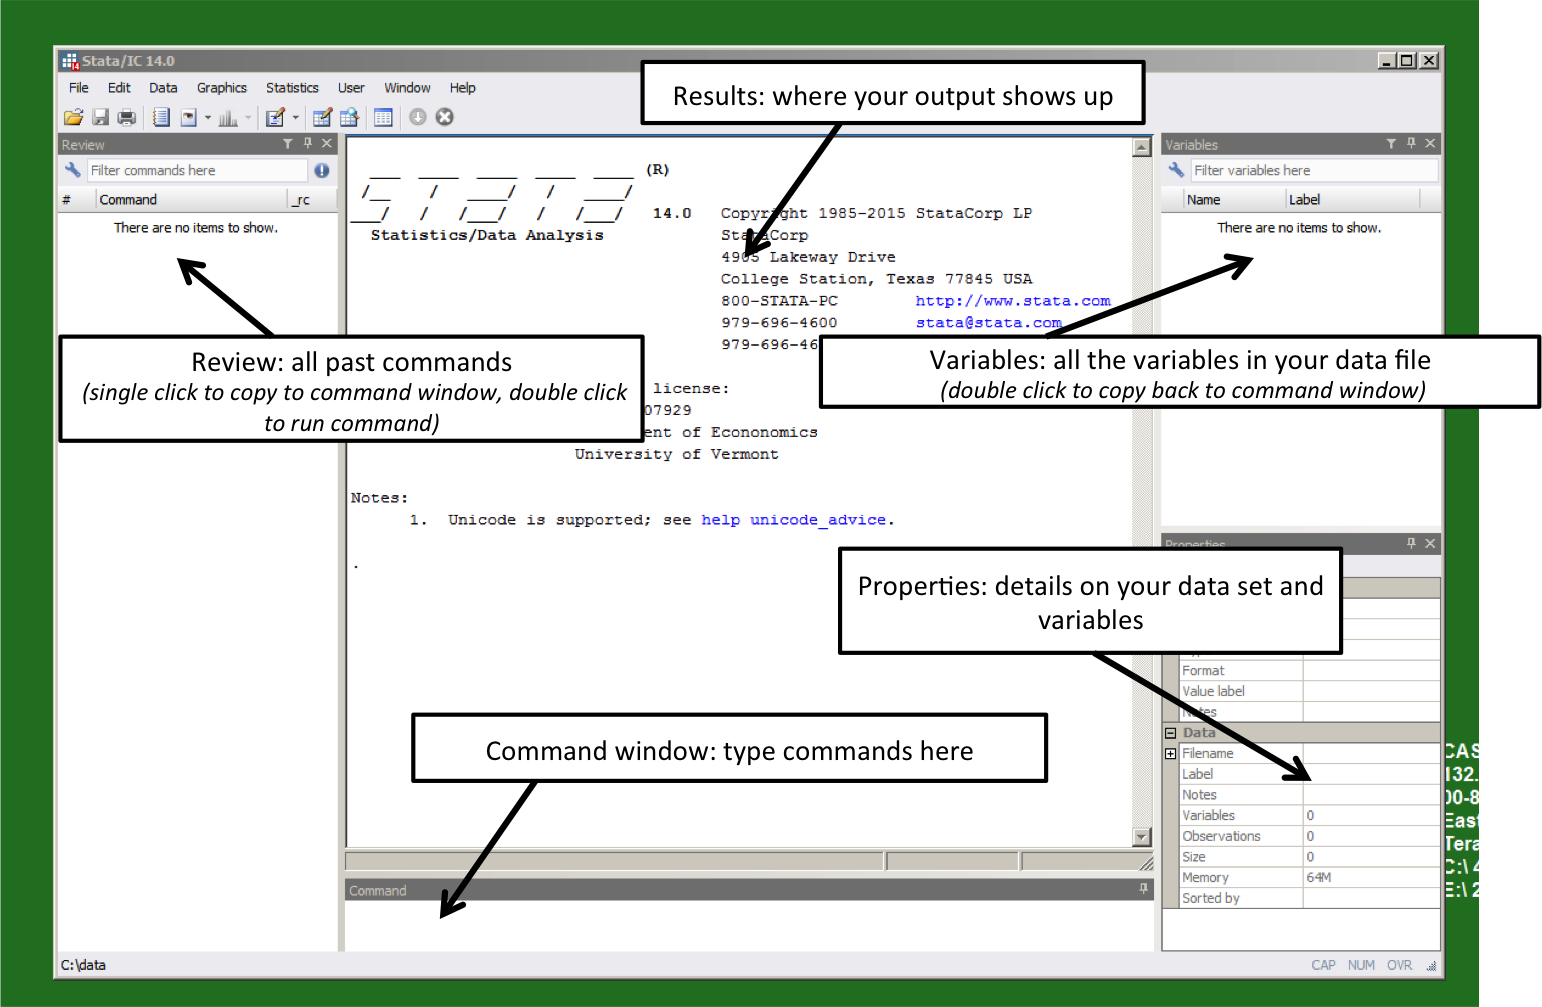
\includegraphics[scale=0.3]{stata1.png}
%\texttt{\{\{\textless{}\ figure\ library="true"\ src="stata1.png"\ title=""\ \textgreater{}\}\}}

You should now have the Stata window open. There is a set of pull down
menus as well as 4 smaller windows: Review, Variables, Results, and
Command.

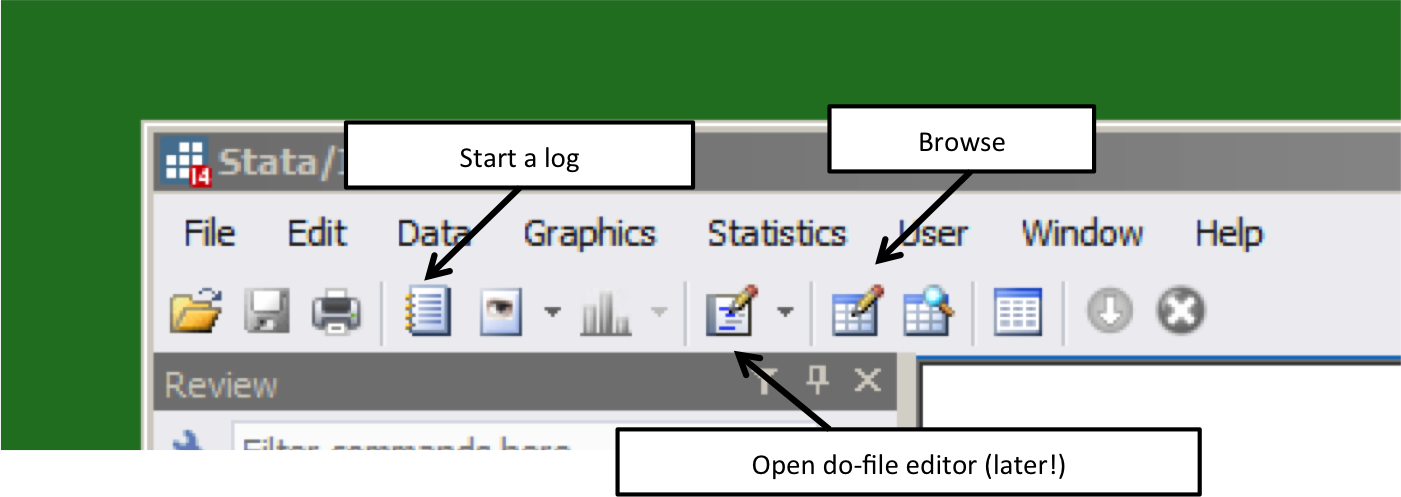
\includegraphics[scale=0.5]{stata2.png}

%\texttt{\{\{\textless{}\ figure\ library="true"\ src="stata2.png"\ title=""\ \textgreater{}\}\}}

Also especially helpful are the following buttons:

\hypertarget{log-files}{%
\subsection*{Log files}\label{log-files}}

If you want to record anything that you do in a Stata session so that
you can look at results or commands later, you need to open a log-file.
A log-file is simply a record of all the commands you enter into Stata
and the output from those commands. The key is to make sure you have a
log file open at the beginning of a Stata session, and to close it once
you have finished, and before you close Stata.

There are three ways you can open a log file:

\begin{enumerate}
\def\labelenumi{\arabic{enumi}.}
\item
  Go to the \textbf{FILE} dropdown menu, choose \textbf{Log}, choose
  \textbf{Begin}. You should see a ``Begin Logging Stata Output'' dialog
  box. Browse to a directory where you can store your log file and type
  in the following file name in the File Name space: \texttt{lab1.log}
\item
  Click on the log icon at the top of the Stata workspace (right of the
  print button). When you click on the log button, the ``Begin Logging
  Stata Output'' dialog box pops up. Name your log file as above.
\item
  You can open a log file by typing the following in the Stata command
  window: \texttt{log\ using\ lab1.log,\ replace}

  The \texttt{,\ replace} is optional. If you add it as an
  \textbf{option}, your new file will overwrite your old one. Or, you
  can add \texttt{,\ append} to add it to the bottom of your old log
  file.
\end{enumerate}

\emph{Tip: Use extension .log, NOT the default .smcl. This will make it
easier for you to edit, cut and paste your log in any text editor.}

Now that you have a log file open, we can start our STATA session.

\hypertarget{opening-data-files}{%
\subsection*{Opening data files}\label{opening-data-files}}

Stata data files end with the extension \texttt{.dta}, and they can only
be read by Stata. You can import text files and excel files into Stata,
and you can export \texttt{.dta} files into text files or Excel files,
but we'll cover this later.

There are three ways to open a data file:

\begin{enumerate}
\def\labelenumi{\arabic{enumi}.}
\item
  Outside Stata, double click on the data file you want to open
\item
  Use the \textbf{FILE/OPEN} drop down menu in Stata and open the data
  set that you copied into your folder. Note that in the command window,
  the \texttt{use} command appears. We'll use that one later.
\item
  Type \texttt{use\ filename.dta,\ clear} into the command window within
  Stata
\end{enumerate}

Download \texttt{driving\_2004.dta}, from Teams and open it. This is a
data file of driving laws, vehicle accidents, and fatalities in the
United States in 2004.

You should now see the list of variables appear in the Variables window,
with the variable name, variable label, and some other information.

\hypertarget{looking-at-data}{%
\subsection*{Looking at data}\label{looking-at-data}}

Let's take a more detailed look at the variables in the dataset.

In the command window type: \texttt{describe}

At the top of the output you will see some overall features of the file,
including the number of variables. Below that you will see a list of
every variable, including the variable name, the ``storage type'' (byte,
float, int, etc.) and the variable label. If you see \texttt{–more–} at
the bottom of your screen, press the space bar to continue
scrolling.\footnote{If you are tired of dealing with the ``more'' issue,
  you can enable \texttt{set\ more\ off} into the command window to
  enable continuous scrolling for your session. If you're just done with
  it, try \texttt{set\ more\ off,\ perm} to enable continuous scrolling
  for this and all future sessions.}

To learn more about the variables and the organization of the data, use
the \texttt{browse} command. Type: \texttt{browse} (or click on the
``browse'' button).

Another approach is to add a variable list to the browse command. Type
the following:

\texttt{browse\ year\ sl70plus\ bac10\ bac08\ gdl}

\emph{Again, note that you can also double click on the variable names
so you don't have to type them all!}

This command directs you to a spreadsheet inside Stata where the data
appears. This looks a lot like an Excel spreadsheet!

Note the following:

\begin{itemize}
\item
  Each observation appears on a separate row of the spreadsheet, which
  represents data from a certain year and a certain state. For example
  the first row is for state 1 (Alabama) in 1980. If you move along the
  row, you can see other characteristics about Alabama in 1980.
\item
  Each variable appears in a separate column, and the name of the
  variable is at the column heading.
\end{itemize}

\begin{quote}
How many observations are there? What type of data set is this?
\end{quote}

\hypertarget{examining-variables}{%
\subsection*{Examining variables}\label{examining-variables}}

Let's look at the variables that are included in the data set. There is
an efficient way to find the names of variables you are interested in.
Suppose you are interested in a variable related to alcohol laws. Type
in:

\texttt{lookfor\ alcohol}

This will give you a list of all the variables that have ``alcohol'' in
either their variable name or variable label. In this case, two
variables appear - \texttt{bac10} and \texttt{bac08}.

You can also experiment with all possible combinations of the col, row,
and cell options, and add the \texttt{nofreq} option to suppress the
number of observations. Use help for details:

\texttt{help\ tab}

When you are analyzing variables, you will want to think carefully about
whether you should be looking at row percentages, column percentages, or
cell percentages.

\begin{center}\rule{0.5\linewidth}{0.5pt}\end{center}

\hypertarget{lab-1}{%
\section*{Lab Exercise 1}\label{lab-1}}
\addcontentsline{toc}{subsection}{Lab Exercise 1}

\emph{First, work through the above steps. Then, work through the 7
questions below.}

\hypertarget{what-do-i-submit}{%
\subsubsection*{What do I submit?}\label{what-do-i-submit}}

\begin{enumerate}
\def\labelenumi{\arabic{enumi}.}
\tightlist
\item
  Your written up answers to exercise questions (1) - (7). This can be
  typed or written out then scanned (or photographed), in any reasonable
  format
\item
  A log file that contains the results from the steps prior to the
  exercise \emph{and} the exercise itself.
\end{enumerate}

\hypertarget{questions}{%
\subsubsection*{Questions}\label{questions}}

\begin{enumerate}
\def\labelenumi{\arabic{enumi}.}
\item
  How many states have graduated drivers license laws (GDLs)? How many
  states have speed limits of 70 mph or higher (including no speed
  limit)?
\item
  What percentage of states with GDLs \emph{and} with low speed limits
  (below 70 mph) have blood-alcohol limits of 0.10 (the more lenient
  level)? \emph{Note that some states have blood-alcohol limit for a
  fraction of a year. If so, consider having a limit of 0.10 in place
  for part of the year as having a limit}
\item
  What is the mean fatality rate per 100 million miles across all
  states? What is the standard deviation?
\item
  What was the fatality rate (deaths per 100 million miles) in Vermont?
  (Vermont is state 46)
\item
  Generate a variable \(Y\) equal to one if a state has a fatality rate
  per 100 million miles that is above the mean, and zero otherwise. What
  is \(E(Y)\)?
\item
  Write a joint probability distribution table for the following two
  random variables: \(X\), a random variable equal to one if a state has
  a speed limit of 70 or greater and zero otherwise (see
  \texttt{sl70plus}), and \(Y\), the random variable developed in the
  previous part.
\item
  \emph{Look up the command \texttt{correlate} in the help files}: What
  is the correlation coefficient between nighttime fatalities per
  100,000 population and weekend accidents per 100,000 population? Why
  might this correlation be so strong?
\end{enumerate}

\end{document}

